
\chapter{Main window}

Next to main tab there are 4 tabs to read the various Modbus resources 
"FC 01 Coils", "FC02 Discrete Inputs", "FC 03 Holding Registers", and "FC04 Input Registers".

\section{FC01 - Coils}

The coils tab allows reading and writing digital outputs with the functions FC01/FC05/FC15.
Read/Loop/Write buttons are unlocked only if the connection to a device has been successfully
opened.

\begin{figure}[H]
\centering
\includegraphics[width=0.85\textwidth]{../Img/Modbus_Client_Coils_00.PNG}
\caption{FC01 - Coils}
\end{figure}

The loop function allows the indicated registers to be read in polling, the polling interval is
configured from the tab "Settings". 
By default, read cells are colored blue if the contents are populated (understood as $>$ 0).
At the top right there are commands to read resources from a group or all resources
of type coils configured in the current profile. The configuration of resources as well as the creation and 
association of groups is described in the chapter \ref{template}.

\newpage

The "Read Coil Range" box is a user-defined range of digital outputs that can be read,
the program will then eventually divide the command into multiple FC01 requests each of n coils
indicated above (in the example below equal to 20). 
It is also possible to force multiple coils (FC15) using the form below 
(Force Multiple Coils) or by importing a previously exported csv file.

Coils set to 1 are colored green if the write is successful.
successful:

\begin{figure}[H]
\centering
\includegraphics[width=0.85\textwidth]{../Img/Modbus_Client_Coils_Write_00.PNG}
\caption{FC05 - Write Coils}
\end{figure}

By enabling the "Live Edit" mode, it is possible to directly edit 
the coils by editing the "Value" column, in this case when editing the row the 
program automatically sends the FC05 command to set the coil to the entered value.

\newpage
\section{FC02 - Discrete inputs}

The Inputs tab allows reading digital inputs with FC02 functions. The Read/Loop buttons
as for the Coils tab are unlocked only if a connection to a device has been successfully
opened. The "Read group" and "Read all" buttons allows to read registers previously configured 
in the custom template (registers are read individually whether or not they are consecutive
with each other).

\begin{figure}[H]
\centering
\includegraphics[width=0.85\textwidth]{../Img/Modbus_Client_Inputs_00.PNG}
\caption{FC02 - Discrete Inputs}
\end{figure}

The "Read Input Range" box is a user-defined range of digital inputs can be read,
the program will then eventually split the command into multiple FC02 requests
each of n inputs specified in the single reads box (in the image above equal to 120).

\newpage
\section{FC03 - Holding registers}

The Holding Registers tab allows you to read and write 16-bit digital 
registers with the functions
FC03/FC06/FC16.

\begin{figure}[H]
\centering
\includegraphics[width=0.85\textwidth]{../Img/Modbus_Client_HoldingReg_00.PNG}
\caption{FC03 - Holding Registers}
\end{figure}

The content of the "Value" field can be displayed in either decimal (DEC) or hexadecimal
(HEX). In the table it is also possible to enable the display of the 
corresponding binary value.
By expanding the window it is possible to display additional information (which is configured
in the template window), to a holding register in fact it is possible to
associate a label to identify its contents or display the value converted to integer/
float/string/etc.. Use the "View" drop-down menu to configure the columns you want to display
in the table as shown in the following image.

\begin{figure}[H]
\centering
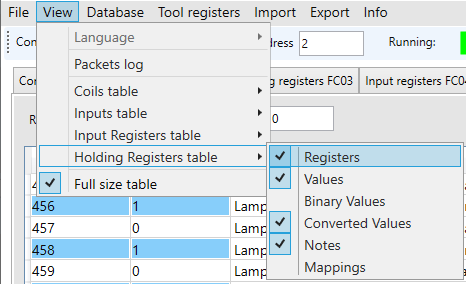
\includegraphics[width=0.40\textwidth]{../Img/Menu_View_Holding.PNG}
\caption{FC03 - View Tab Holding Registers}
\end{figure}

With the "Read Holding Register Range" box, it is possible to read a register range defined
by the user (also > 123), the program will then eventually split the command into multiple
FC03 requests of n registers specified in the box above (in image 120)
and populate the table with all the requested registers.

By checking the "Live Edit" flag, it is possible to send the register write automatically
by editing a cell in the "Value", "Binary Value" or "Converted Value" columns. The
"Live edit" is very useful for editing displayed registers.

\begin{figure}[H]
\centering

\includegraphics[width=0.40\textwidth]{../Img/ModBus_Client_HoldingReg_Live.PNG}
\caption{FC03 - Live edit}
\end{figure}

Note that changes in the "Value" column are sent with the function FC06
(write single register), changes to the "Binary Value" column are converted from
binary and always sent as FC06 while changes to the "Converted Value" column
are sent as FC06 or FC16 depending on the data type (the function 
FC16 is used
for 32- or 64-bit integer or float variables). In the value column you can also enter 
values in hexadecimal; if the display is already in hexadecimal, the value entered will be considered
always hexadecimal, while in the decimal display, prepend a "0x" or "x" or postpone an "h"
to indicate that the value you want to send is written in hexadecimal.


The displayed table can be exported in .csv or .json format with the "Export" button at the bottom
right. Tables exported to csv can be imported and sent to the slave with the "Import" button.
This function is convenient when you want to copy a memory map from one PLC to another or simply
export a backup that can be restored at any time.

\begin{figure}[H]
\centering
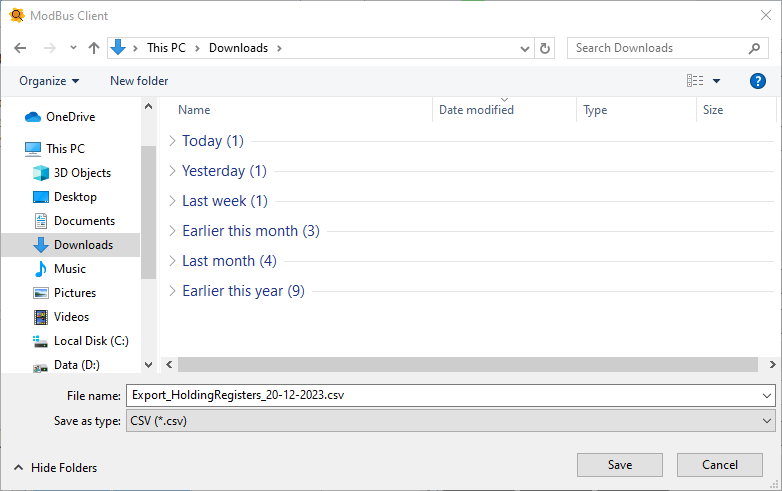
\includegraphics[width=0.70\textwidth]{../Img/ModBus_Client_HoldingReg_Import.PNG}
\caption{FC03 - CSV import}
\end{figure}

\newpage
\section{FC04 - Input registers}

The Input Registers tab allows you to read 16-bit registers with the FC04 functions. The buttons
Read/Loop as for the other tabs are unlocked only if the connection to a device is
successful.

\begin{figure}[H]
\centering
\includegraphics[width=0.85\textwidth]{../Img/Modbus_Client_InputReg_00.PNG}
\caption{FC04 - Input Registers}
\end{figure}

The content of the "Value" field can be displayed in either decimal (DEC) or hexadecimal
(HEX) representation. The value in binary is also shown next to it. By expanding the window, it is possible to
display additional information (which is configured in the template window). To a
register in fact, it is possible to associate a label to identify its contents or to display the value
converted to integer/float/string/etc.. See the Template section for further clarification of this part.
With the "Read Input Register Range" box, it is possible to read a user-defined register range
(even > 123), the program will then eventually split the command into multiple FC04 requests
to populate the table with all the requested registers.

\begin{figure}[H]
\centering
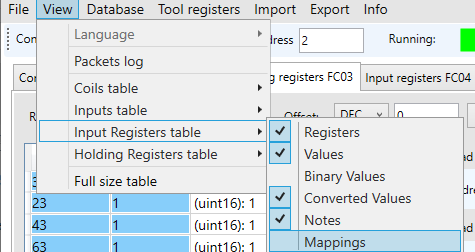
\includegraphics[width=0.60\textwidth]{../Img/Menu_View_InputReg.PNG}
\caption{FC04 - Input Registers}
\end{figure}

As with holding registers, it is possible to select from the view menu 
which columns to show to the user.

\newpage
\section{Diagnostic}

In the diagnostics tab, diagnostic commands can be sent to the queried device, 
be aware
that not all devices respond to the FC08 function.

\begin{figure}[H]
\centering
\includegraphics[width=0.85\textwidth]{../Img/Modbus_Client_Diagnostic_00.PNG}
\caption{FC08 - Diagnostic}
\end{figure}

Supported FC08 functions:

\begin{verbatim}
    - 00 Return Query Data
    - 01 Restart Comunications Option
    - 02 Return Diagnostic Register
    - 03 Change ASCII Input Delimeter
    - 04 Force Listen Only Mode
    - 10 Clear Counters and Diagnostic Register
    - 11 Return Bus Message Count
    - 12 Return Bus Comunication Error Count
    - 13 Return Bus Exception Error Count
    - 14 Return Slave Message Count
    - 15 Return Slave No Response Count
    - 16 Return Slave NAK Count
    - 17 Return Slave Busy Count
    - 20 Clear Overrun Counter and Flag
\end{verbatim}

Use this tab also if you need to build Modbus telegrams manually.
In case of RTU connection use the CRC button to calculate and append the CRC16
according to the Modbus protocol specification. On serial comunication infact
the slave checks the CRC to see if the packet contains transmission errors,
so if you don't append the CRC the slave ignores the command and doesn't respond
to any request.
